% Name: DFA minimization
% Description: A five-state DFA for (a|b)*abb above its minimal equivalent, in which the equivalent states A and C are merged into one.
% Tags: DFA minimization, equivalent states, Myhill-Nerode, finite automaton

\usetikzlibrary{automata, arrows.meta}

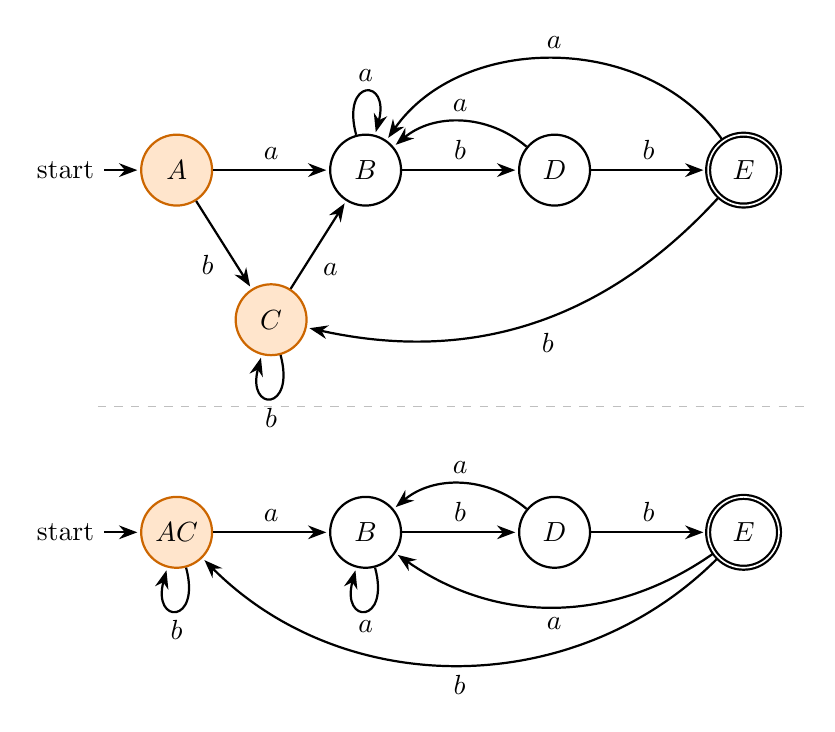
\begin{tikzpicture}[shorten >=1pt, auto, thick, >={Stealth},
    every state/.style={minimum size=9mm, inner sep=1pt}, same/.style={fill=orange!20, draw=orange!80!black}]
  % Before: A and C go to B on a and to C on b, and neither accepts, so they are equivalent.
  \node[state, initial, same] (A) at (0,0) {$A$};
  \node[state] (B) at (2.4,0) {$B$};
  \node[state, same] (C) at (1.2,-1.9) {$C$};
  \node[state] (D) at (4.8,0) {$D$};
  \node[state, accepting] (E) at (7.2,0) {$E$};
  \path[->] (A) edge node {$a$} (B) edge[swap] node {$b$} (C)
    (B) edge[loop above] node {$a$} () edge node {$b$} (D)
    (C) edge[swap] node[pos=0.4] {$a$} (B) edge[loop below] node {$b$} ()
    (D) edge[bend right=40, swap] node {$a$} (B) edge node {$b$} (E)
    (E) edge[bend right=55, swap] node {$a$} (B) edge[bend left=30] node {$b$} (C);

  % After: four states, one per equivalence class.
  \node[state, initial, same] (AC) at (0,-4.6) {$AC$};
  \node[state] (B2) at (2.4,-4.6) {$B$};
  \node[state] (D2) at (4.8,-4.6) {$D$};
  \node[state, accepting] (E2) at (7.2,-4.6) {$E$};
  \path[->] (AC) edge[loop below] node {$b$} () edge node {$a$} (B2)
    (B2) edge[loop below] node {$a$} () edge node {$b$} (D2)
    (D2) edge[bend right=40, swap] node {$a$} (B2) edge node {$b$} (E2)
    (E2) edge[bend left=35] node {$a$} (B2) edge[bend left=45] node {$b$} (AC);
  \draw[gray!50, dashed, thin] (-1,-3) -- (8,-3);
\end{tikzpicture}
